%File Generated with PyPaper
\documentclass[aps,prl,amsmath,amssymb,superscriptaddress,notitlepage,groupedaddress]{revtex4-1}
\usepackage{graphicx}
\usepackage{dcolumn}
\usepackage{stackengine}
\usepackage[section]{placeins}
\usepackage[dvipsnames*,svgnames]{xcolor}
\usepackage{verbatim}
\usepackage[position=bottom,caption=false,captionskip=3pt,font=normalsize,subrefformat=simple,labelformat=simple]{subfig}
\renewcommand{\thesubfigure}{(\alph{subfigure})}
\usepackage{listings}
\usepackage{mathtools}
\usepackage{todonotes}
\usepackage{amsmath}
\usepackage{chngcntr}
\usepackage{bm}
\usepackage{url}
\def\UrlBreaks{\do\/\do-}
\newcommand {\framedgraphic}[2] {\begin{frame}{#1}\begin{center}\includegraphics[width=\textwidth,height=0.8\textheight,keepaspectratio]{#2}\end{center}\end{frame}}\usepackage[breaklinks]{hyperref}
\usepackage{tabularx}
\usepackage{soul}
\hypersetup{
colorlinks,
linkcolor={blue!100!black},
citecolor={blue},
urlcolor={blue!80!black}}
\lstset{basicstyle=\small\ttfamily,columns=flexible,breaklines=true}\newcommand{\fakesection}[1]{\par\refstepcounter{section}\sectionmark{#1}\addcontentsline{toc}{section}{\protect\numberline{\thesection}#1}}\def\equationautorefname~#1\null{#1\null}
\raggedbottom\usepackage[bottom]{footmisc} \makeatletter \def\p@section{} \def\p@subsubsection{} \makeatother\begin{document}
\title{\texttt{bayesim}: a tool for fast model fitting with Bayesian inference}
\author{Rachel Kurchin}
\affiliation{Department of Materials Science \& Engineering, Massachusetts Institute of Technology, 77 Massachusetts Avenue, Cambridge, MA 02139, USA}
\author{Giuseppe Romano}
\affiliation{Department of Mechanical Engineering, Massachusetts Institute of Technology, 77 Massachusetts Avenue, Cambridge, MA 02139, USA}
\author{Tonio Buonassisi}
\email{buonassi@mit.edu}
\affiliation{Department of Mechanical Engineering, Massachusetts Institute of Technology, 77 Massachusetts Avenue, Cambridge, MA 02139, USA}

\begin{abstract}
Target journal: Computer Physics Communications
\end{abstract}

\maketitle

\section*{Introduction}
  There are a plethora of examples across diverse scientific and engineering fields of mathematical models used to simulate the results of experimental observations. In many cases, there are input parameters to these models which are difficult to determine via direct measurement, and it is desirable to invert the numerical model -- that is, use the experimental observations to determine values of the input parameters. Bayesian inference is a fruitful framework within which to do such fitting, since the resulting posterior probability distribution over the parameters of interest can give rich insights into not just the most likely values of the parameters, but also uncertainty about these values and the potentially complicated ways in which they can covary to give equally good fits to observations.

  We have previously demonstrated the value of a Bayesian approach in using automated high-throughput temperature- and illumination-dependent current-voltage measurements (JVTi) to fit material/interface properties and defect recombination parameters in photovoltaic (PV) absorbers~\cite{SnSJoule,FeBayes}. In cases such as these, when the data model is not a simple analytical equation but rather a computationally intensive numerical model, efficient, nonredundant sampling of the parameter space when computing likelihoods becomes critical to making the fit feasible.

  In this work, we introduce \texttt{bayesim}, a Python-based code that utilizes adaptive grid sampling to perform Bayesian parameter estimation. We discuss the structure of the code, its implementation, and provide several examples of its usage. While the authors' expertise is in the realm of semiconductor physics and thus the examples herein are drawn from that space, we also discuss the general characteristics of a problem amenable to this approach so that researchers from other fields might adopt it as well.

\section*{Model}
  \todo[inline]{Should this section title actually just be ``Technical Background`` as well perhaps?}

 Bayes' Theorem is a relationship between conditional probabilities. It states

 \begin{equation}
   \begin{split}
     \label{Eq:1001}
     P(H|E)=\frac{P(H)P(E|H)}{P(E)}
   \end{split}
 \end{equation}

 where the notation $P(A|B)$ indicates the probability of $A$ being true given that $B$ is true. $H$ is a \textit{hypothesis} and $E$ the observed \textit{evidence}. $P(H)$ is termed the \textit{prior}, $P(E|H)$ the \textit{likelihood}, $P(H|E)$ the \textit{posterior}, and $P(E)$ is a normalizing constant. If there are $n$ pieces of evidence, this can generalize to an iterative process where

 \begin{equation}
   \begin{split}
     \label{Eq:2}
     P(H|\{E_1,E_2,...E_n\}) = \frac{P(H|\{E_1,E_2...E_{n-1}\})P(E_n|H)}{P(E_n)}
   \end{split}
 \end{equation}

 In a multidimensional parameter estimation problem, each hypothesis $H$ is a tuple of possible values for the fitting parameters, i.e. a point in the parameter space, while the evidence $E$ is an observed output of a measurement as a function of various experimental conditions.

 In order to compute a likelihood, a model capable of simulating that observed output as a function of both the fitting parameters and the experimental conditions is required. In \texttt{bayesim}, likelihoods are calculated for each point in parameter space using a Gaussian where the argument is the difference between observed and simulated output at that point, and the standard deviation is the sum of experimental uncertainty and model uncertainty. The experimental uncertainty is a number provided by the user that quantifies any noise/irreproducibility inherent to the measurement, while the model uncertainty is calculated by \texttt{bayesim} and reflects the sparseness of the parameter space grid, i.e. how much simulated output changes from one grid point to another.

 \begin{figure}
   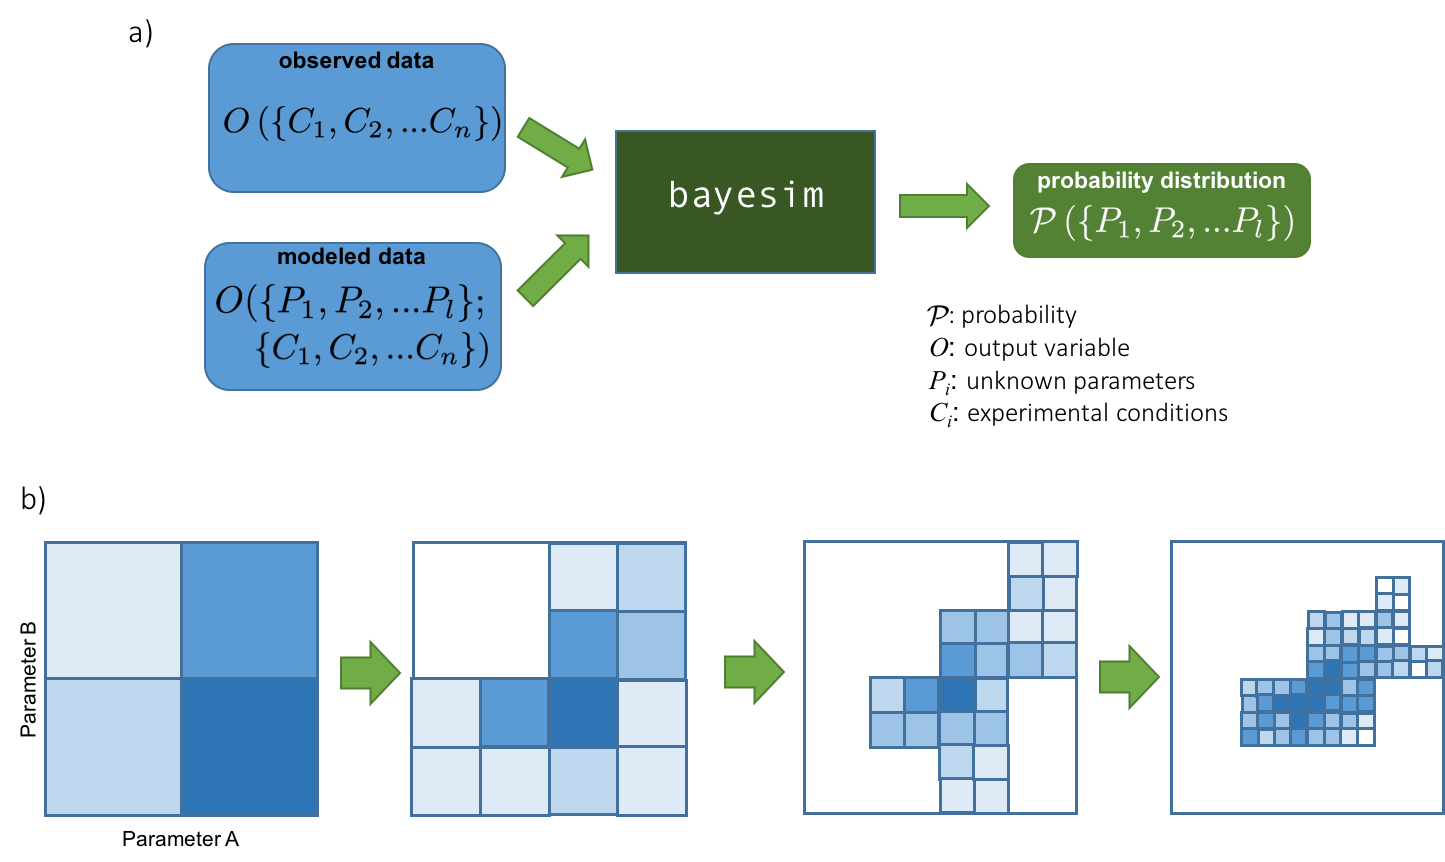
\includegraphics[width=0.7\columnwidth]{figure_1.png}
   \caption{(Figure copied from docs website for now, will make a publication-appropriate version)}
   \label{fig1}
 \end{figure}

 A high-level summary of what \texttt{bayesim} does is shown in ~\autoref{fig1}. Part (a) is a flowchart showing that observed (as a function of experimental conditions $\{C\}$ and simulated (as a function of fitting parameters $\{P\}$ and experimental conditions $\{C\}$) outputs are compared to produce a probability distribution over $\{P\}$. Part (b) schematically indicates the adaptive grid sampling approach for a hypothetical two-dimensional parameter space, wherein grid boxes exceeding some threshold probability are subdivided and lower-probability regions discarded, allowing attainment of a high fitting precision without needing to sample the entire parameter space at the same high density.

\section*{Software Architecture and Interface}

  \begin{figure}
    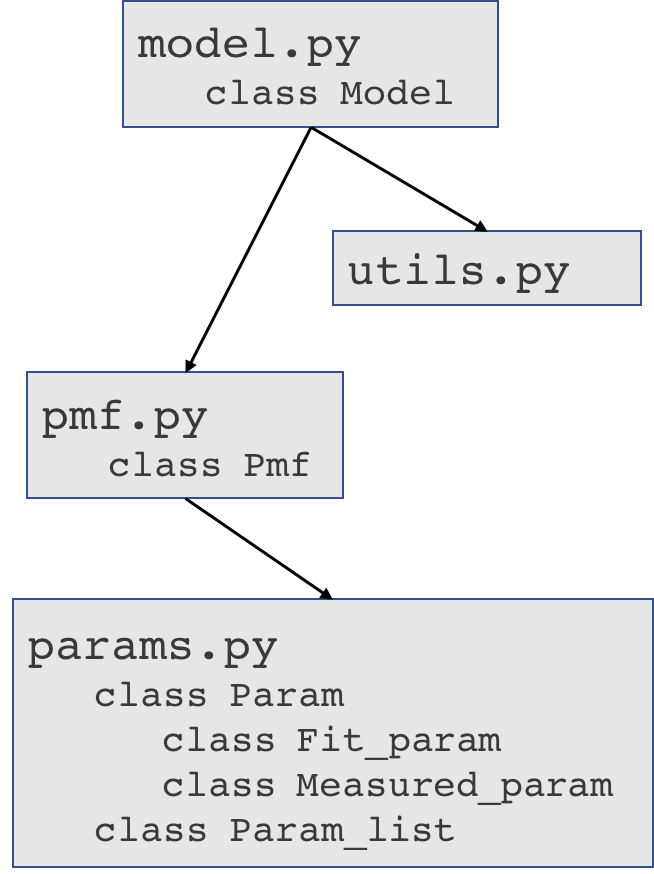
\includegraphics[width=0.7\columnwidth]{structure.png}
    \caption{\texttt{bayesim} software structure, indicating class definitions, internal and external dependencies, and interfaces.}
    \label{structure}
  \end{figure}

  The structure of \texttt{bayeim} is shown in ~\autoref{structure}. Detailed and up-to-date documentation of classes, functions, and example applications is maintained online.~\cite{docs}

  \subsection{Structure}

    The top-level object with which users interact is implemented in the \texttt{Model} class. The \texttt{params} module defines classes to store information about the various types of parameters (fitting parameters, experimental conditions, and measured output) while the \texttt{Pmf} class stores the probability distribution and implements the manipulations required for Bayesian updates.

  \subsection{Interfaces}
    The most flexible way to interact with \texttt{bayesim} is via Python scripting or through literate programming in a Jupyter notebook. There is also a command line interface (CLI) for users less familiar with coding in Python.

  \subsection{Dependencies}
    \texttt{bayesim} relies on a variety of external open-source packages. These include \texttt{numpy}~\cite{numpy} and \texttt{scipy}~\cite{scipy} for a variety of mathematical functions and vectorized implementations, \texttt{joblib}~\cite{joblib} for simple parallelism, \texttt{deepdish}~\cite{deepdish} for saving and loading HDF5 files, \texttt{pandas}~\cite{pandas} for data manipulation, and \texttt{matplotlib}~\cite{mpl} for visualization.

\section*{Application Examples}
  \subsection{Ideal Diode Model}
    \begin{itemize}
      \item validation example - ``observed'' data is just generated using the model and we show we can recover the correct input parameters
      \item figure 3 showing PMF
    \end{itemize}

  \subsection{SnS Solar Cell}
    \begin{itemize}
      \item more practical example - replicating fit from Joule paper
      \item figure 4 showing PMF and comparison of JV curves
    \end{itemize}


\section*{Conclusions}
 talk about broader applicability of approach

\section*{Acknowledgements}

\section*{Appendix}
 \begin{itemize}
   \item include minimal code to run ideal diode example
   \item link to Github repo (which has installation instructions and documentation as well as list of planned future features)
  \end{itemize}

\bibliography{biblio}
\bibliographystyle{ieeetr}

\end{document}
